\documentclass[9pt,twocolumn,twoside]{osajnl}
%% Please use 11pt if submitting to AOP
% \documentclass[11pt,twocolumn,twoside]{osajnl}

\journal{josab} % Choose journal (ao, aop, josaa, josab, ol, optica, pr)

% See template introduction for guidance on setting shortarticle option
\setboolean{shortarticle}{false}
% true = letter / tutorial
% false = research / review article
% (depending on journal).

\usepackage{subcaption}
\usepackage{tikz}
\usepackage{mathtools}

\usetikzlibrary{patterns,decorations.pathreplacing}
\usetikzlibrary{arrows.meta}
\usetikzlibrary{shapes.arrows, fadings}

% Fixes bracket spacing
\let\originalleft\left
\let\originalright\right
\renewcommand{\left}{\mathopen{}\mathclose\bgroup\originalleft}
\renewcommand{\right}{\aftergroup\egroup\originalright}

\providecommand{\df}{\textrm{d}} % Roman d for differentials
\newcommand{\diff}[3][\hspace{-0.5pt}]{\frac{\df^{#1}#2}{\df{#3}^{#1}}} % Derivatives
\newcommand{\pdiff}[3][\hspace{-0.5pt}]{\frac{\partial^{#1}#2}{\partial{#3}^{#1}}} % Partial derivatives
\newcommand{\Es}{E_{\textrm{sat}}} % Saturation energy
\newcommand{\FT}[1]{\mathcal{F}\left\{ #1 \right\}} % Fourier transform
\newcommand{\FTi}[1]{\mathcal{F}^{-1}\left\{ #1 \right\}} % Inverse Fourier transform

\providecommand{\bigO}[1]{\ensuremath{\mathop{}\mathopen{}\mathcal{O}\mathopen{}\left(#1\right)}} % Big O notation

\DeclareMathOperator{\sech}{sech}

\title{Predicting instabilities of a tuneable ring laser with an iterative map model}

\author[1]{Brady Metherall}
\author[2,*]{C. Sean Bohun}

\affil[1]{Mathematical Institute, University of Oxford, Radcliffe Observatory Quarter, Woodstock Rd, Oxford OX2 6GG, UK}
\affil[2]{Facutlty of Science, University of Ontario Institute of Technology, 2000 Simcoe St N, Oshawa, ON L1G 0C5, Canada}

\affil[3]{brady.metherall@maths.ox.ac.uk}
\affil[4]{sean.bohun@ontariotechu.ca}

%% To be edited by editor
% \dates{Compiled \today}

%\ociscodes{(140.3490) Lasers, distributed feedback; (060.2420) Fibers, polarization-maintaining;(060.3735) Fiber Bragg gratings.}

%% To be edited by editor
% \doi{\url{http://dx.doi.org/10.1364/XX.XX.XXXXXX}}

\begin{abstract}
	We propose a nonlinear iterative map for tuneable ring lasers. Using the generalized nonlinear Schr\"odinger equation, expressions for the transformations undergone by the laser pulse are derived for each of the five components (gain, loss, dispersion, modulation, and nonlinearity) within the laser cavity. These transformations are then iteratively composed to give the overall effect of one round trip of the cavity. We first examine the linear version of the model which we solve analytically. Then the full nonlinear model is investigated numerically. The nonlinear model is able to exhibit wave breaking as well as modulation instability. We highlight the rich landscape and sharp divide for a particular plane of the parameter space.
\end{abstract}

\setboolean{displaycopyright}{true}

\begin{document}

\maketitle

\section{Introduction}
\label{sec:intro}
Tuneable lasers have the ability to vary the frequency of their output by up to about 100 nanometres~\cite{bohun2015, burgoyne2010, yamashita2009}. This ability to vary the frequency leads to applications such as optical coherence tomography~\cite{bohun2015, burgoyne2014, yamashita2009}, coherent anti-Stokes Raman spectroscopy~\cite{burgoyne2014}, deep tissue multi-photon microscopy~\cite{chung2017}, and diagnostics of ultrafast processes~\cite{burgoyne2014, silfvast2004}. Tuneable lasers are usually constructed in a ring with five main components: output coupler, chirped fibre Bragg grating (CFBG), modulator, Er-doped fibre, and pump laser. A typical ring laser cavity is depicted in Fig.~\ref{fig:cavity}. Due to the high power and short duration of the pulses, the Kerr nonlinearity plays a crucial role in the dynamics within the cavity.

Several effects arise within the cavity due to the interplay of dispersion, modulation, and the nonlinearity~\cite{bohun2015, coen1997, lapre2019, meng2020, shao2019, woodward2018}. The two effects of most interest for this paper are wave breaking, and modulation instability. Wave breaking causes the leading edge of a pulse to be red shifted, and the trailing edge blue shifted (in the anomalous dispersion regime, the effect is reversed) to the point that a shock is developed~\cite{anderson1992, rothenberg1989a, rothenberg1989b, tomlinson1984, tomlinson1985}. The shifts in frequencies cause the pulse to become more rectangular in the frequency domain with a linear chirp over most of the pulse. In optics, wave breaking manifests from self-phase modulation (SPM) which is a direct effect of the Kerr nonlinearity causing the pulse to interfere with itself. New frequencies are then generated which induces the rectangular profile~\cite{agrawal2013, woodward2018}. Outside of optics, wave breaking occurs in other areas with nonlinear waves such as plasmas, heat propagation, transmission lines, and fluid dynamics~\cite{rothenberg1989b}. Modulation instability---which typically arises in the anomalous dispersion regime---is the other effect that will be of interest. However, in the presence of multiple frequencies, modulation instability can emerge in the normal dispersion regime as well through cross-phase modulation and four-wave mixing~\cite{agrawal1987, agrawal2013, haelterman1992}. Modulation instability causes a wave to break into short pulses, and can cause a laser to lose coherence~\cite{agrawal1987, coen1997, haelterman1992}. Within a ring laser cavity wave breaking and modulation instability can become parasitic leading to an unstable and unsustainable pulse. This gives rise to the need of understanding the rich landscape of the parameter space, and determining design principles to guarantee the ring laser is stable and sustainable~\cite{bohun2015, burgoyneemail, finot2008, lapre2019, woodward2018}.

\begin{figure}[tbp]
	\centering
	% !TeX root = ./Tuneable_Lasers.tex

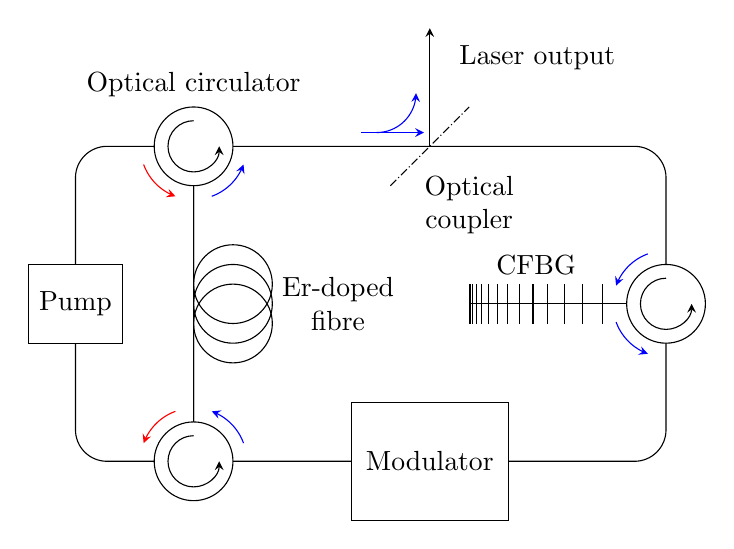
\begin{tikzpicture}
% Two laser loops
\draw [rounded corners=4mm] (0,0) rectangle ++(6,4);
\draw [rounded corners=4mm] (0,0) rectangle ++(-1.5,4);

% Gain
\draw (0.5,2.25) circle (0.5cm);
\draw (0.5,2) circle (0.5cm) node [anchor=west,xshift=0.5cm,align=center] {Er-doped \\ fibre};
\draw (0.5,1.75) circle (0.5cm);

% Modulator and pump
\filldraw[fill=white, draw=black] (2,-0.75) rectangle ++(2,1.5) node [midway] {Modulator};
\filldraw[fill=white, draw=black] (-2.1,1.5) rectangle ++(1.2,1) node [midway] {Pump};

% Coupler and output
\draw[-stealth] (3,4) -- (3,5.5) node [pos=0.75,anchor=west,xshift=0.25cm] {Laser output};
\draw[densely dashdotted] (2.5,3.5) -- (3.5,4.5) node [pos=1,anchor=north,yshift=-0.75cm,align=center] {Optical \\ coupler};

% Circulators
\filldraw[fill=white, draw=black] (6,2) circle (0.5cm);
\draw[->,>=stealth] (6,2.325) arc (90:360:0.325cm);

\filldraw[fill=white, draw=black] (0,0) circle (0.5cm);
\draw[->,>=stealth] (0,0.325) arc (90:360:0.325cm);

\filldraw[fill=white, draw=black] (0,4) circle (0.5cm) node [anchor=south,align=center,yshift=0.5cm] {Optical circulator};
\draw[->,>=stealth] (0,4.325) arc (90:360:0.325cm);

% Arrows
\draw [->,>=stealth,domain=20:70,blue] plot ({0.675*cos(\x)}, {0.675*sin(\x)});
\draw [->,>=stealth,domain=110:160,red] plot ({0.675*cos(\x)}, {0.675*sin(\x)});
\draw [->,>=stealth,domain=110:160,blue] plot ({6+0.675*cos(\x)}, {2+0.675*sin(\x)});
\draw [->,>=stealth,domain=200:250,blue] plot ({6+0.675*cos(\x)}, {2+0.675*sin(\x)});
\draw [->,>=stealth,domain=200:250,red] plot ({0.675*cos(\x)}, {4+0.675*sin(\x)});
\draw [->,>=stealth,domain=290:340,blue] plot ({0.675*cos(\x)}, {4+0.675*sin(\x)});

\draw [->,>=stealth,domain=270:360,blue] plot ({2.325+0.5*cos(\x)}, {4.675+0.5*sin(\x)});
\draw [->,>=stealth,blue] (2.125, 4.675-0.5) -- (2.325+0.6, 4.675-0.5);

% Grating
\draw (5.5,2) -- (3.5,2) node [pos=0.5,anchor=south,yshift=0.25cm,xshift=-0.15cm] {CFBG};
\foreach \i in {0,...,13}
	\draw (3.5 + \i*\i/100,1.75) -- (3.5 + \i*\i/100,2.25);

\end{tikzpicture}
	\caption{Typical cavity of a fibre ring laser~\cite{burgoyne2014, chung2017, lapre2019, shao2019}. The laser pulses travel clockwise around each loop.}
	\label{fig:cavity}
\end{figure}

In this paper, we will build an iterative map model for the evolution of a laser pulse as it travels though the cavity. In Section~\ref{sec:modelling}, we will briefly review previous mathematical models for ring lasers. Then, we will present our own iterative map model in Section~\ref{sec:model}, as well as non-dimensionalize the model and introduce four dimensionless parameters that govern the dynamics of the system. We will then examine the results of our model in Section~\ref{sec:results}---first solving the model analytically, by assuming the absence of the nonlinearity, then numerically solving the full nonlinear model. We will identify a sharp boundary in the parameter space separating the region of stability, and the region where modulation instability degrades the pulse. Finally, the concluding thoughts and possible ideas for future work are given in Section~\ref{sec:conclusion}.

\section{Modelling Efforts}
\label{sec:modelling}
The standard equation for studying nonlinear optics is the nonlinear Schr\"odinger equation (NLSE),
\begin{align}
	\pdiff{A}{z} &= - i \frac{\beta_2}{2}\pdiff[2]{A}{T} + i \gamma |A|^2 A.
	\label{eq:smallnlse}
\end{align}
Here, $A = A(T, z) : \mathbb{R}^2 \mapsto \mathbb{C}$ is the complex pulse amplitude, $\beta_2 \in \mathbb{R}$ is the second order dispersion, and $\gamma \in \mathbb{R}$ is the coefficient of nonlinearity. In practice, the NLSE, \eqref{eq:smallnlse}, lacks a few key terms, thus, it is often generalized by adding amplification and loss (occasionally higher order terms are added as well). These additions give the generalized nonlinear Schr\"{o}dinger equation (GNLSE)~\cite{agrawal2013, bohun2015, finot2008, peng2018, shtyrina2017, yarutkina2013},
	\begin{align}
	\pdiff{A}{z} &= - i \frac{\beta_2}{2}\pdiff[2]{A}{T} + i \gamma |A|^2 A + \frac{1}{2}g(A) A - \alpha A,
	\label{eq:nlse}
\end{align}
where $g(A)$ is an amplifying term due to the gain, and $\alpha \in \mathbb{R}^+$ is the loss due to scattering and absorption.

The GNLSE has many applications in nonlinear optics and fibre optic communications, however, in laser physics typically a modulation term is also added to ensure mode-locking, this yields the master equation of mode-locking~\cite{haus1984, haus1975, haus1986, haus1992, haus2000, tamura1996, usechak2005},
\begin{align}
	\pdiff{A}{z} &= - i \frac{\beta_2}{2}\pdiff[2]{A}{T} + i \gamma |A|^2 A + \frac{1}{2}g(A) A - \alpha A - M(T).
	\label{eq:meml}
\end{align}
No analytic solution is known for \eqref{eq:meml}---even after making the assumptions that the gain is constant, and the modulation is quadratic~\cite{haus1984, haus1975, haus1996}. However, by neglecting certain terms of \eqref{eq:meml} analytic solutions can be found~\cite{burgoyne2014, haus1975, haus1986, haus1991, haus1992, haus1996, tamura1996, usechak2005}. See Haus~\cite{haus2000} for a comprehensive description and history of the theory of mode-locked lasers.

\subsection{Discrete Models}
\label{sec:discrete}
Unfortunately, the master equation, \eqref{eq:meml}, is not completely representative of the underlying physics within our laser cavity. It is assumed in \eqref{eq:meml} that each process affects the pulse continuously within the cavity. As highlighted by Fig.~\ref{fig:cavity}, this can be a poor assumption. Within the cavity, each effect is localized to its corresponding component: almost all of the dispersion happens within the CFBG~\cite{agrawal2002}, the pulse is only amplified within the Erbium-doped fibre, \emph{et cetera}. Thus, a better model is one where we consider a simplified version of \eqref{eq:meml} for each component. Solving these simplified differential equations yields an algebraic expression for the effect of each individual component. The relations can then be functionally composed to give an iterative map for the effect of one round trip of the cavity.

Such a method was first proposed in 1955 by Cutler~\cite{cutler1955} while analyzing a microwave regenerative pulse generator. His method was adapted for mode-locked lasers in 1969 by Siegman and Kuizenga~\cite{kuizenga1970a, kuizenga1970b, kuizenga1970, siegman1969}. The effects of the nonlinearity would not be considered until Martinez \emph{et al.}~\cite{martinez1984, martinez1985} modelled passively mode-locked lasers. This issue has recently been readdressed by Burgoyne~\cite{burgoyne2014} in the literature for tuneable lasers. In each of these models the effect of each block is described by a transfer function.

Despite the development of discrete, block style models, several short-comings exist. None of the previous models have contained every component within a laser cavity---either the nonlinearity or the modulation have been omitted. Each component of a tuneable plays a pivotal role and the laser will not function correctly without the inclusion of all of the components. Another drawback is that the functional operations of some of the components used in their models are phenomenological. While these functions are chosen based on the observed output, they are not necessarily consistent with the underlying physics. Finally, the previous models have been unsuccessful in exhibiting the instabilities described in Section~\ref{sec:intro}.

\section{Model Derivation}
\label{sec:model}
Using the idea of a discrete model presented Section~\ref{sec:modelling}\ref{sec:discrete}, we derive our model from the GNLSE, \eqref{eq:nlse}; however, in the case of the modulation we consider the exact functional form to be determined by the laser operator. To accomplish this we follow the method described in Section~\ref{sec:modelling}\ref{sec:discrete}; we neglect all terms but one on the right side of \eqref{eq:nlse} and solve the simplified differential equations.

To proceed we must choose the form of the amplification term, $g(A)$. We assume the gain has the form
\begin{align}
	g(A) &= \frac{g_0}{1 + E / \Es},& E &= \int_{-\infty}^\infty |A|^2 \, \df T,
	\label{eq:energy}
\end{align}
where $g_0$ is a small signal gain, $E$ is the energy of the pulse, and $\Es$ is the energy at which the gain begins to saturate~\cite{haus1984, shtyrina2017, silfvast2004}. This reduces \eqref{eq:nlse} to
\begin{align}
	\pdiff{A}{z} &= \frac{g_0 A}{2 \left( 1 + E / \Es \right)}.
\end{align}
By assuming the energy entering the gain fibre is $E_g$ and the energy after travelling through the gain fibre of length $L_g$ is $E_{\text{out}}$, we find the energy after amplification is
\begin{align}
	\label{eq:engain}
	E_{\text{out}} &= \Es W \left( \frac{E_g}{\Es} \exp( E_g / \Es ) \exp( g_0 L_g ) \right),
\end{align}
where $W$ is the Lambert $W$ function. Rewriting \eqref{eq:engain} in terms of the pulse gives
\begin{align}
	G(A) &= \left( \frac{\Es}{E_g} W \left( \frac{E_g}{\Es} \exp( E_g / \Es ) \exp( g_0 L_g ) \right) \right)^{1/2} A
	\label{eq:gainform}
\end{align}
for the amplification of the pulse within the Er-doped fibre. Repeating this process for the loss, dispersion, and nonlinearity yields
\begin{align}
	L(A) &= (1 - R) \exp( - \alpha L_T )A, \\
	D(A) &= \FTi{\exp( i \omega^2 L_D\beta_2/2 ) \FT{A}}, \\
	F(A) &= A \exp( i \gamma |A|^2 L_f ),
\end{align}
where $R$ is the reflectivity of the output coupler (depending on the layout of the laser cavity the loss may instead take the form $L(A) = R \exp( - \alpha L_T )A$), $L_T$ is the total length of the laser circuit, $L_D$ is the length of the dispersive medium, $L_f$ is the length of fibre between the amplifier and the output coupler, and $\mathcal{F}$ denotes the Fourier transform. Finally, we must consider the modulation. Here, we assume the pulse is modulated by an electro-optic modulator. This gives the freedom of choosing the profile of the modulation how ever the operator sees fit. For simplicity the representation is taken as the Gaussian
\begin{align}
	M(A) &= \exp( -T^2 / 2 T_M^2 ) A,
	\label{eq:modform}
\end{align}
where $T_M$ is the characteristic width of the modulation. This assumption is not particularly restrictive. Calcaterra and Boldt~\cite{calcaterra2008a} have shown that a sum of Gaussian functions can approximate any square integrable function. Therefore, our solution extends to any continuous, bounded modulation function. Additionally, it is common to use a saturable absorber in place of a modulator. In this case, \eqref{eq:modform} can freely be replaced by~\cite{lapre2019, meng2020}
\begin{align}
	S(A) &= 1 - \frac{q_0}{1 + |A|^2 / P_\text{sat}},
\end{align}
where $q_0$ is the modulation depth, $|A|^2$ is the instantaneous power of the pulse, and $P_\text{sat}$ is the saturation power.

\subsection{Non-Dimensionalization}
Non-dimensionalization is a technique used in mathematical modelling to better understand the relative importance of different processes within a system. In essence, we scale all variables by typical values of the system based on the geometry and boundary conditions (see, for example,~\cite{howison2005}). Doing so `factors' the dimensional units out of the problem, leaving only dimensionless equations with dimensionless parameters. The magnitude of the dimensionless parameters characterizes the dominant dynamics of the system---much like how fluid flow can be described with only the Reynolds number. The structure of each process in the laser can be better understood by re-scaling the time, energy, and amplitude by the convenient scalings:
\begin{align}
	T &= T_M \widetilde{T},& E &= \Es \widetilde{E},& A &= \left( \frac{\Es}{T_M} \right)^{1/2} \widetilde{A}.
\end{align}

Revisiting the process maps \eqref{eq:gainform}--\eqref{eq:modform} yields the new, non-dimensional, mappings---after dropping the tildes---
\begin{align}
	G(A) &= \left(E_g^{-1} W \left( a E_g \textrm{e}^{E_g}\right) \right)^{1/2} A, & F(A) &= A \exp( i b |A|^2), \nonumber \\
	D(A) &= \FTi{\exp( i s^2 \omega^2 ) \FT{A}}, & L(A) &= h A, \label{eq:effects} \\
	M(A) &= \exp( -T^2 / 2 ) A, \nonumber
\end{align}
with the four dimensionless parameters, as defined by the values in Table~\ref{tab:values},
\begin{equation}
	\begin{aligned}
		a &= \exp( g_0 L_g ) \sim 8 \times 10^3, & 
		h &= (1 - R) \exp( - \alpha L_T) \sim 0.04, \\
		b &= \gamma L_f \frac{\Es}{T_M} \sim 1, & s &= \left( \frac{\beta_2 L_D}{2 T_M^2} \right)^{1/2} \sim 0.2.
		\label{eq:ndparam}
	\end{aligned}
\end{equation}
Here, $a$ is a measure of the strength of the gain fibre, $h$ is the loss due to absorption and the output coupler, $b$ is the ratio of the frequency shift due to the Kerr nonlinearity to the width of the pulse, and $s$ is the ratio of the effectiveness of the CFBG to the width of the pulse. Furthermore, notice that in this non-dimensional form, the modulation has no associated parameter, and each of the other processes in \eqref{eq:ndparam} have their own independent, non-dimensional parameter.

% Table of parameter values
\begin{table*}[tbp]
	\centering
	\caption{Range of parameter values (taken from~\cite{agrawal2013, burgoyne2014, burgoyneemail, tamura1996, usechak2005}).}
 	\label{tab:values}
 	\begin{tabular}{clll}
		\hline\noalign{\smallskip}
		Symbol & Parameter & Value & Units \\
		\hline\noalign{\smallskip}
		$\alpha$ & Absorption of fibre & $10^{-4}$--$0.3$ & m$^{-1}$ \\
		$\beta_2^f$ & Fibre dispersion & $-50$--$50$ & ps$^2$/km \\
		$\gamma$ & Fibre nonlinearity & $0.001$--$0.01$ & W$^{-1}$ m$^{-1}$ \\
		$\beta_2^g L_D$ & Grating dispersion & $10$--$2000$ & ps$^2$ \\
		$L_T$ & Length of cavity & $10$--$100$ & m \\
		\vspace*{-2mm} $L_f$ & Length of fibre between & $0.15$--$1$ & m \\
		& gain and output coupler & & \\
		$L_g$ & Length of gain fibre & $2$--$3$ & m \\
		$T_M$ & Modulation Time & $15$--$150$ & ps \\
		$R$ & Reflectivity of optical coupler & $0.1$--$0.9$ & -- \\
		$\Es$ & Saturation energy & $10^3$--$10^4$ & pJ \\
		$g_0$ & Small signal gain &  $1$--$10$ & m$^{-1}$ \\
		\noalign{\smallskip}\hline
	\end{tabular}
\end{table*}

\subsection{Combining the Effects}
\label{sec:effects}

\begin{figure}[tbp]
	\centering
	\includegraphics{Figures/Evo}
	\caption{Evolution of the envelope during one round trip of the cavity at equilibrium. The pulse decays due to the output coupler, disperses due to the CFBG, is modulated by the modulator, and finally, is amplified by the gain fibre (the envelope is unaltered by the nonlinearity). Note, the $z$ axis is not to scale.}
	\label{fig:cavityevo}
\end{figure}

Now that we have the algebraic effect of each section of the cavity, we are ready to take the composition of the maps to give the effect of one round trip of the cavity. Thus, we must now consider the order of the components. As we are most interested in the output of the laser cavity, we shall start with the loss. We then pass the pulse through the CFBG followed by the modulator. The pulse then travels through the Er-doped fibre to be amplified, and finally we consider the effect of the nonlinearity. The nonlinearity must immediately follow the gain in this model---this is where the nonlinearity will have the largest effect since this is where the pulse is most energetic. Note, the permutation of the components is indeed important as the operators do not, in general, commute---unlike the models described in Section~\ref{sec:modelling}\ref{sec:discrete}. Moreover, we prefer the loss to follow the gain and nonlinearity as we wish to minimize the length over which the nonlinearity has an effect, and maximize the output power. Functionally we denote one round trip of the cavity by
\begin{align}
	\mathcal{L}(A) = F(G(M(D(L(A))))).
	\label{eq:order}
\end{align}
 The pulse after one complete circuit of the laser cavity is then returned back into the cavity to restart the process. A steady solution to this model is one in which the envelope and chirp are unchanged after traversing every component in the cavity---we are uninterested in the phase due to the nature of experimental measurements. That is, such that $\mathcal{L}(A) = A \textrm{e}^{i \phi}$---for some $\phi \in \mathbb{R}$. An example of the evolution of the envelope during one round trip of the laser cavity can be found in Fig.~\ref{fig:cavityevo}.

\section{Results}
\label{sec:results}
We split the results into two subsections. In the following subsection we investigate the low nonlinearity limit, and in Section~\ref{sec:results}\ref{sec:nlresults} we look at the full nonlinear model.

\subsection{Linear Solution}
By neglecting the effect of the nonlinearity, that is, $b = 0$, a solution can be found analytically. We proceed by assuming the solution will take the form of a chirped Gaussian. There are a few reasons for this; the solution to the models presented in~\cite{cutler1955, siegman1969, kuizenga1970a, martinez1984, martinez1985} were Gaussian, the equilibrium shape will be highly correlated to the modulation function, and since a Gaussian is a fixed point of the Fourier transform. Furthermore, this form is chosen because it resembles the envelope and linear chirp expected from the literature~\cite{burgoyne2014, haus1975, haus1996, haus2000, usechak2005}.

\begin{figure}[tbp]
	\centering
	\includegraphics{Figures/Sample_Gauss}
	\caption{Linearly chirped Gaussian pulse, \eqref{eq:A0}.}
	\label{fig:samplegauss}
\end{figure}

Consider the pulse
\begin{align}
	A = \sqrt{P} \exp \left( -(1 + iC) \frac{T^2}{2 \sigma^2} \right) \textrm{e}^{i \phi_0},
	\label{eq:A0}
\end{align}
where $P$ is the peak power, $C$ is the chirp, $\sigma^2$ is the variance, and $\phi_0$ is the phase (Fig.~\ref{fig:samplegauss}). By computing $\mathcal{L}(A)$ using \eqref{eq:order}, and equating to $A \textrm{e}^{i \phi}$, we obtain the conditions
\begin{align}
	\frac{\sigma^4}{1 - \sigma^2} &= (\sigma^2 + 2 C s^2)^2 + 4 s^4, \label{eq:sigrelation} \\
	\frac{C}{1 - \sigma^2} &= C + 2 \frac{s^2}{\sigma^2} (1 + C^2), \label{eq:chirprelation} \\
	1 &= \frac{W(a E_g \textrm{e}^{E_g})}{E_g} h^2 (1 - \sigma^2)^{1/2} \label{eq:energyrelation}
\end{align}
for \eqref{eq:A0} to be in equilibrium. Manipulating \eqref{eq:sigrelation} and \eqref{eq:chirprelation} we are able to eliminate the chirp, and find an expression in terms of $\sigma$ only, that is,
\begin{align}
	\sigma^8 + 4 s^4 \sigma^6 - 20 s^4 \sigma^4 + 32 s^4 \sigma^2 - 16 s^4 = 0. \label{eq:var}
\end{align}
As \eqref{eq:var} is a quartic in $\sigma^2$, it has an analytic solution, namely,
\begin{equation}
	\begin{split}
		\sigma^2 = \sqrt{2} s \left( s^6 + 3s^2 + \sqrt{4 + s^4} \left( 1 + s^4 \right) \right)^{1/2} & \\
		- s^4 - s^2 & \sqrt{4 + s^4}.
		\label{eq:equilvar}
	\end{split}
\end{equation}
Additionally, we find the chirp to be
\begin{align}
	C = \frac{\sigma^4 - \left( \sigma^8 - 16 s^4 \left( 1 - \sigma^2 \right)^2 \right)^{1/2}}{4 s^2 \left( 1 - \sigma^2 \right)},
	\label{eq:chirp}
\end{align}
in terms of $s$ and $\sigma^2$. Moreover, we can obtain the energy of the pulse entering the gain fibre, $E_g$, from \eqref{eq:energyrelation}, and thus, the equilibrium energy at the output coupler. Doing so gives
\begin{align}
	E &= \frac{\log \left( a h^2 \left( 1 - \sigma^2 \right)^{1/2} \right)}{1 - h^2 \left( 1 - \sigma^2 \right)^{1/2}}.
	\label{eq:analenergy}
\end{align}
By equating the energy of the pulse in \eqref{eq:A0} and \eqref{eq:analenergy}, the peak power is found to be
\begin{align}
	P &= \frac{\log \left( a h^2 \left( 1 - \sigma^2 \right)^{1/2} \right)}{\sqrt{\pi} \sigma \left( 1 - h^2 \left( 1 - \sigma^2 \right)^{1/2} \right)}.
	\label{eq:analpower}
\end{align}

The nature of \eqref{eq:var}--\eqref{eq:analpower} makes it difficult to work with. However, by asymptotically expanding \eqref{eq:var}--\eqref{eq:analpower} in terms of the dispersion parameter, $s$, we find the simpler relations
\begin{align}
	\sigma^2 &\sim 2s(1 - s) + \bigO{s^3}, \\
	C &\sim 1 - s + \frac{1}{2}s^2 + \bigO{s^3}, \\
	E &\sim \frac{\log (a h^2)}{1 - h^2} - \frac{1}{1 - h^2} \left( 1 + \frac{h^2 \log(a h^2)}{1 - h^2}  \right) s + \bigO{s^2}, \label{eq:maxenergy} \\
	P &\sim \frac{\log(ah^2)}{\sqrt{2 \pi}(1 - h^2)} s^{-1/2} + \bigO{s^{1/2}},
\end{align}
in the case $s \rightarrow 0$. And,
\begin{align}
	\sigma^2 &\sim 1 - \frac{1}{4}s^{-4} + \frac{3}{8}s^{-8} + \bigO{s^{-12}}, \label{eq:siginfty}\\
	C &\sim \frac{1}{2}s^{-2} - \frac{3}{8}s^{-6} + \bigO{s^{-10}},
\end{align}
in the case $s \rightarrow \infty$. We have no asymptotic expansion of the energy or peak power as $s \rightarrow \infty$ since in this limit the gain is unable to balance the energy lost due to modulation, as indicated by the logarithm in \eqref{eq:analenergy}. Expanding the condition $a h^2 (1 - \sigma^2)^{1/2} > 1$, from \eqref{eq:analenergy}, using \eqref{eq:siginfty} (for a first-order approximation), we find 
\begin{align}
	s^* = \left( \frac{a h^2}{2} \right)^{1/2}
\end{align}
is the maximum value of $s$ to facilitate a sustainable pulse.

Our linearized model indeed exhibits a solution of the same form as previous linear models. However, by including the effects of the nonlinearity we uncover the rich interplay between dispersion, modulation, and nonlinearity.

\subsection{Nonlinear Solution and Instability}
\label{sec:nlresults}
In this iterative map model---as well as within the laboratory---we must specify the input pulse. One of the most common forms is a hyperbolic secant~\cite{coen1997, finot2008, rothenberg1989b, tomlinson1984}, which we assume has the exact form
\begin{align}
	A_0 = \Gamma \sech \left( 2 T \right) \textrm{e}^{i \pi / 4},
	\label{eq:nlA0}
\end{align}
where $\Gamma$ is a normalizing factor chosen so the pulse has the initial energy $E_0$, which we take as $E_0 = 0.1$, unless specified otherwise. Using \eqref{eq:nlA0} as a seed, we simulate the pulse as it travels around the cavity using $2^{18}$ points, and a time span of 16.

\begin{figure}[tbp]
	\centering
	\begin{subfigure}{\columnwidth}
		\centering
		\includegraphics{Figures/Chirp}
		\caption{Chirp.}
		\label{fig:chirp}
	\end{subfigure} \\
	\vspace{3mm}
	\begin{subfigure}{\columnwidth}
		\centering
		\includegraphics{Figures/FT}
		\caption{Fourier transform.}
		\label{fig:ft}
	\end{subfigure}
	\caption{Chirp and Fourier transform at equilibrium (500 round trips) initiated by \eqref{eq:nlA0} for two values of $b$, the nonlinearity parameter ($a = 8 \times 10^3$, $h = 0.04$, $s = 0.2$, and $E_0 = 0.1$).}
	\label{fig:chirpft}
\end{figure}

In Fig.~\ref{fig:chirpft} we show the chirp and Fourier transform of the pulse \eqref{eq:nlA0} once it has reached equilibrium for the nominal parameter values given in \eqref{eq:ndparam}, and an additional $b$ value. In this nonlinear case, we find that the equilibrium pulse is no longer Gaussian---as evidenced by the Fourier transforms. Notice that compared to the linear case, higher frequency modes are introduced due to the nonlinearity, giving a bi-modal appearance. Moreover, we find the pulse is linearly chirped near the peak, but, in the tails, $|T| > 1$, the chirp begins to saturate---consistent with the experimental results~\cite{chen2008, rothenberg1989b, tomlinson1985}. As the nonlinearity parameter, $b$, is increased, the chirp increases more sharply across the pulse, and saturates at a larger value. Also, the two lobes in the Fourier transform become more pronounced and further apart, and the pulse becomes more rectangular. However, after a critical point, SPM plays a more substantial role, leading to modulation instability. This phenomenon is highlighted in Fig.~\ref{fig:breakevo}. By increasing the nonlinearity, and decreasing the dispersion we find the pulse begins to `breathe'. During the first two dozen round trips of the cavity, the SPM compounds and becomes too parasitic to the pulse. This in turn induces modulation instability, and degrades the pulse, until the pulse is no longer stable or sustainable. On the other hand, having a more moderate value of $b$, the pulse is able to equilibrate even with a less favourable, random, initial pulse (Fig.~\ref{fig:convevo}), as in~\cite{meng2020}. The pulse is able to shed the initial left lobe ($T = -1 / 2$) because of dispersion and modulation, and a central lobe ($T = 0$) is formed and is able to grow due to the gain medium. This then allows the pulse to come to equilibrium very quickly. Furthermore, since the intensity of the initial pulse is relatively small, the effect of SPM is negligible during the first few round trips which allows the laser to select preferable modes. The preferable modes then get amplified which stabilizes the pulse. From this, it is clear the initial shape of the pulse is much less important than the initial energy of the pulse, $E_0$, or the strength of the nonlinearity, $b$.

\begin{figure}[tbp]
	\centering
	\includegraphics{Figures/Break}
	\caption{Example of a pulse destabilizing from the initial pulse \eqref{eq:nlA0} ($a = 8 \times 10^3$, $h = 0.04$, $b = 1.6$, $s = 0.1$, and $E_0 = 0.1$).}
	\label{fig:breakevo}
\end{figure}

\begin{figure}[tbp]
	\centering
	\includegraphics{Figures/Conv}
	\caption{Example of a pulse coming to equilibrium from noise ($a = 8 \times 10^3$, $h = 0.04$, $b = 1.0$, $s = 0.1$, and $E_0 = 0.1$).}
	\label{fig:convevo}
\end{figure}

We now turn our attention to a more quantitative analysis, and characterize the stability of a laser by exploring the parameter space. We focus on the $s$--$b$ plane in particular since $a$ and $h$ effect only the amplitude of the pulse, whereas the interplay of dispersion and nonlinearity give rise to the instabilities. Additionally, as mentioned, a conservative initial energy will effect the dynamics much less than a more intense pulse since the nonlinearity will be negligible while coming to equilibrium. To identify the stability of a pulse we examine the relative change in the pulse's envelope between consecutive round trips of the cavity. We compute this error by
\begin{align}
	\Delta = \frac{\| |\mathcal{L}^n(A_0)| - |\mathcal{L}^{n-1}(A_0)| \|_2}{\| \mathcal{L}^{n-1}(A_0) \|_2},
	\label{eq:error}
\end{align}
where
\begin{align}
	\| f \|_2^2 \coloneqq \int_{-\infty}^\infty |f|^2 \, \df T,
\end{align}
and $n$ is chosen to be sufficiently large to guarantee the pulse reaches equilibrium or degrades due to modulation instability---we use $n = 500$ in our experiments. We take the modulus of the pulse since we are only interested in the evolution of the envelope because of the methods used experimentally. We plot the error in Fig.~\ref{fig:error}. It is clear the parameter space is split into two distinct regions, divided by an incredibly sharp and complex boundary. In the upper-left region the error is $\bigO{1}$; here, the nonlinearity is too strong, and the SPM induces modulation instability. In the lower-right region we find the opposite behaviour---the pulse reaches an equilibrium state and is stable. The increase in dispersion, coupled with modulation, allows the laser to balance the nonlinear effects. The error in this region is on the order of machine precision, or slightly higher due to the discretization.

\begin{figure}[tbp]
	\centering
	\includegraphics{Figures/ParamSpaceErr}
	\caption{Relative error of a pulse's envelope between round trips 499 and 500 ($a = 8 \times 10^3$, $h = 0.04$, and $E_0 = 0.1$).}
	\label{fig:error}
\end{figure}

Also of interest is the energy of the pulse at equilibrium, which we compute numerically by \eqref{eq:energy}. Recall from \eqref{eq:order}, this energy is immediately before passing through the output coupler, and so the energy of each pulse emitted by the laser is $(1 - h^2) E$, and $h^2 E$ remains in the cavity. We plot the energy in the $s$--$b$ plane in Fig.~\ref{fig:energy}. Unsurprisingly, we find the same sharp boundary as we saw in Fig.~\ref{fig:error}. In the unstable region (upper-left) the energy is relatively small. Since the pulse is not sustainable in this region it is not able to foster prominent modes, thus, the intensity is low across the entire pulse. In the stable region (lower-right) we find that the energy smoothly decays as both $b$ and $s$ increase, with the contours being hyperbolic-esque. As $s$ increases, more energy is lost due to modulation since the tails of the pulse become larger. Similarly, as $b$ increases, high frequencies generated by SPM are reduced by our choice of modulation function. From this, we find that a more energetic laser requires weaker dispersion, however, the nonlinearity must be correspondingly low, otherwise modulation instability will destroy the pulse. Moreover, the maximum energy, which occurs in the limit that both $s$ and $b$ go to zero, is slightly larger than 2.5. With our choice of parameters, \eqref{eq:maxenergy} predicts an energy of 2.55 at the origin, inline with Fig.~\ref{fig:energy}.

\begin{figure}[tbp]
	\centering
	\includegraphics{Figures/ParamSpaceEnergy}
	\caption{Energy of the pulse after 500 round trips ($a = 8 \times 10^3$, $h = 0.04$, and $E_0 = 0.1$).}
	\label{fig:energy}
\end{figure}

Finally, we briefly investigate the effect the order of the components has on the dynamics. In Section~\ref{sec:model}\ref{sec:effects} we justified the order of the gain, nonlinearity, and loss, but, just assumed dispersion preceded modulation. Here, we consider the effect of swapping the dispersion and modulation components. The energy landscape (Fig.~\ref{fig:energyswitch}) is as we would expect. In the previous case of having modulation following dispersion, more energy is removed from the pulse tails. Whereas, having modulation first, more of this energy remains in the cavity. This has the effect of making the laser more powerful than in the previous case, which in turn increases the size of the unstable region. Comparing with Fig.~\ref{fig:energy}, the unstable upper-left region spreads farther rightward, and the energy is larger in the stable region---especially farther away from the origin. Lastly, once again, the energy at the origin is somewhat larger than 2.5, as predicted by \eqref{eq:maxenergy}.

\begin{figure}[tbp]
	\centering
	\includegraphics{Figures/ParamSpaceEnergySwitch}
	\caption{Energy of the pulse after 500 round trips with dispersion and modulation swapped ($a = 8 \times 10^3$, $h = 0.04$, and $E_0 = 0.1$).}
	\label{fig:energyswitch}
\end{figure}

\section{Conclusion}
\label{sec:conclusion}
Expanding upon the ideas originally proposed by Cutler~\cite{cutler1955}, and Kuizenga and Siegman~\cite{kuizenga1970, kuizenga1970a, siegman1969}, we developed a nonlinear iterative map model for tuneable ring lasers. We recovered linearly chirped Gaussian solutions in the case of a Gaussian modulation function when omitting the nonlinearity. Moreover, the solution of the linear model can easily be extended to any modulation function using results of~\cite{calcaterra2008a}. In contrast, with the inclusion of the nonlinearity we were able to recover wave breaking and modulation instability, and found a sharp boundary of stability. This phenomenon has been demonstrated in a laboratory setting~\cite{agrawal2013, anderson1992, finot2008, rothenberg1989b, tomlinson1985}, but, has proven difficult to predict with simple mathematical models~\cite{meng2020}.

It is of interest to analyze the nonlinear model analytically using an asymptotic expansion for small values of the nonlinearity parameter, $b$. Doing so would provide insight to how the nonlinearity impacts the linearized solution to better understand the manifestation of wave breaking and modulation instability.

\section*{Acknowledgement.}

Portions of this work were presented at The V AMMCS International Conference in 2019, ``A new method of modelling tuneable lasers with functional composition'' \cite{metherallammcs}. BM acknowledges the support provided by the EPSRC Centre for Doctoral Training in Industrially Focused Mathematical Modelling (EP/L015803/1).

\section*{Disclosures.}
The authors declare no conflicts of interest.

\bibliography{Ref}

\end{document}
